\section{HSV}
Nella strutturazione del progetto ci è venuto molto naturale andare a lavorare con una scala di colori HSV. Ma perchè non applicare un filtraggio basato su RGB?
Come noto nella letteratura, nell'ambito dell'\textit{image recognition} è usuale il problema di andare a mascherare un colore piuttosto che un altro, come nel nostro caso.
Potremmo voler trovare, sempre per esempio, oggetti rosso, scannerizzando nell'immagine solamente colori (255,0,0) nella scala RGB; con questo approccio andremmo ad applicare una condizione troppo stringente ai colori.
Si potrebbe pensare, come soluzione a questa condizione parecchio stringente, di trovare colori in un range di rossi, come per esempio {(130,0,0);(255,0,0)}: il problema comunque persisterebbe proprio per il fatto che il rosso è ottenuto come combinazione di più colori primari, e non come un solo singolo colore.
Potremmo pensare a questo istante di andare a fondo del problema, applicando 

So at this point we could continue going down this path, changing the RGB range for all three primary colour values; but it honestly requires a lot of effort to cover all our bases and even if somehow we do manage to get a reasonable range setup it’s very likely we’ll end up with a lot of noise in the fields we detect.

We need a method that doesn’t have to many parameters in order to simplify our detection space. This is where HSV comes into the picture (excuse the pun).

TODO: completare

\begin{figure}
	\centering
	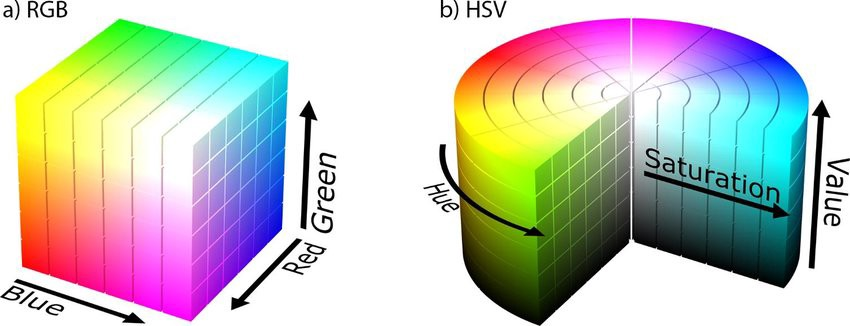
\includegraphics[width=0.5\textwidth]{Immagini/HSV_RGB.jpeg}
	\caption{RBG vs HSV}
	\label{fig:TrustCam}
\end{figure}

Lo standard per 
\section{Frecce o cerchi?}
\section{Maschere}
\section{Erosione e dilatazione}